\documentclass[9pt]{beamer}
\usepackage[utf8]{inputenc}
\usepackage[T1]{fontenc}
\usepackage[english]{babel}
\usepackage{xcolor}
\usepackage{csquotes}
\usepackage{expl3}
\usepackage[style=numeric, sorting=none]{biblatex}   % Using biblatex with unsrt style
\addbibresource{bib.bib}  % Add your .bib file here

\usepackage{booktabs}
\usepackage{amsmath}  % Added this package for better math formatting
\usetheme[
  workplace=mu,
]{MU}

\title[Discovered Policy Optimisation]{Discovered Policy Optimisation}
\author[H. Adamove]{Hugo Adamove\texorpdfstring{\\}{, }}
\institute[MU]{IV125 Formela lab seminar}
\date{\today}
\subject{Presentation Subject}
\keywords{the, presentation, keywords}

\begin{document}

\frame{\titlepage}

\begin{frame}[plain]
  \section{Motivation}
  \vfill
  \begin{center}
    \Huge \textbf{Motivation}
  \end{center}
  \vfill
\end{frame}



\begin{frame}{Trust Region Learning and PPO}
  \begin{block}{Trust Region Learning (TRL) Update}
    \begin{equation}
      \pi_{i+1} = \arg \max_{\pi' \in \Pi} \mathbb{E}_{s \sim \pi_i, a \sim \pi'} \left[ A_{\pi_i}(s,a) \right] - C_{\pi_i} \, D_{\text{KL}}(\pi_i, \pi'),
    \end{equation}
    where
    \begin{itemize}
        \item   \(C_{\pi_i}\) is a constant dependent on \(\pi_i\) only,
        \item \( \Pi \) is the set of all possible policies.
    \end{itemize}
    \vfill
    \pause
     Schulman et al. \cite{trl2015} showed that this update guarantees monotonic improvement in the expected return \( \eta\):
    \[
    \eta(\pi_{i+1}) \geq \eta(\pi_i)
    \]
  \end{block}

\pause

\vfill
  
  \begin{block}{PPO Update}
    \begin{equation}
      \pi_{i+1} = \arg \max_{\pi' \in \Pi} \mathbb{E}_{s \sim \pi_i, a \sim \pi'} \left[ L_{\text{clip}} \right],
    \end{equation}
    where
    \[
 L_{\text{clip}} = \min \Bigg ( A_{\pi_i}(s,a)\ r(\pi'), \,  A_{\pi_i}(s,a)\ \text{CLIP} \Big( r(\pi'), 1 - \epsilon, 1 + \epsilon \Big) \Bigg).
    \]
  \end{block}
\end{frame}

\begin{frame}{PPO's "Paradox"}
  \begin{itemize}
    \item PPO stabilizes training and achieves SOTA performance across various tasks (Henderson et al., 2018; Berner et al., 2019) \cite{berner2019dota}.
    
    \vspace{1em}  % Adds space between points for better distribution
\pause

    \item PPO’s theoretical foundations remain limited to heuristic “proof by analogy” rather than a rigorous guarantee of monotonic improvement.
    
    \vspace{1em}  % Adds space between points for better distribution
    
\pause
    \item Despite being based on TRL principles, PPO fails to constrain update size, violating core TRL principles (Wang et al., 2020; Engstrom et al., 2020) \cite{wang2020truly}.
    
\pause
    \vspace{1em}  % Adds space between points for better distribution

   \item How can PPO’s empirical success be theoretically justified?
  \end{itemize}
\end{frame}

\begin{frame}[plain]
  \section{Mirror Learning}
  \vfill
  \begin{center}
    \Huge \textbf{Mirror Learning}
  \end{center}
  \vfill
\end{frame}


\begin{frame}{Mirror Learning}
  \begin{figure}
    \centering
    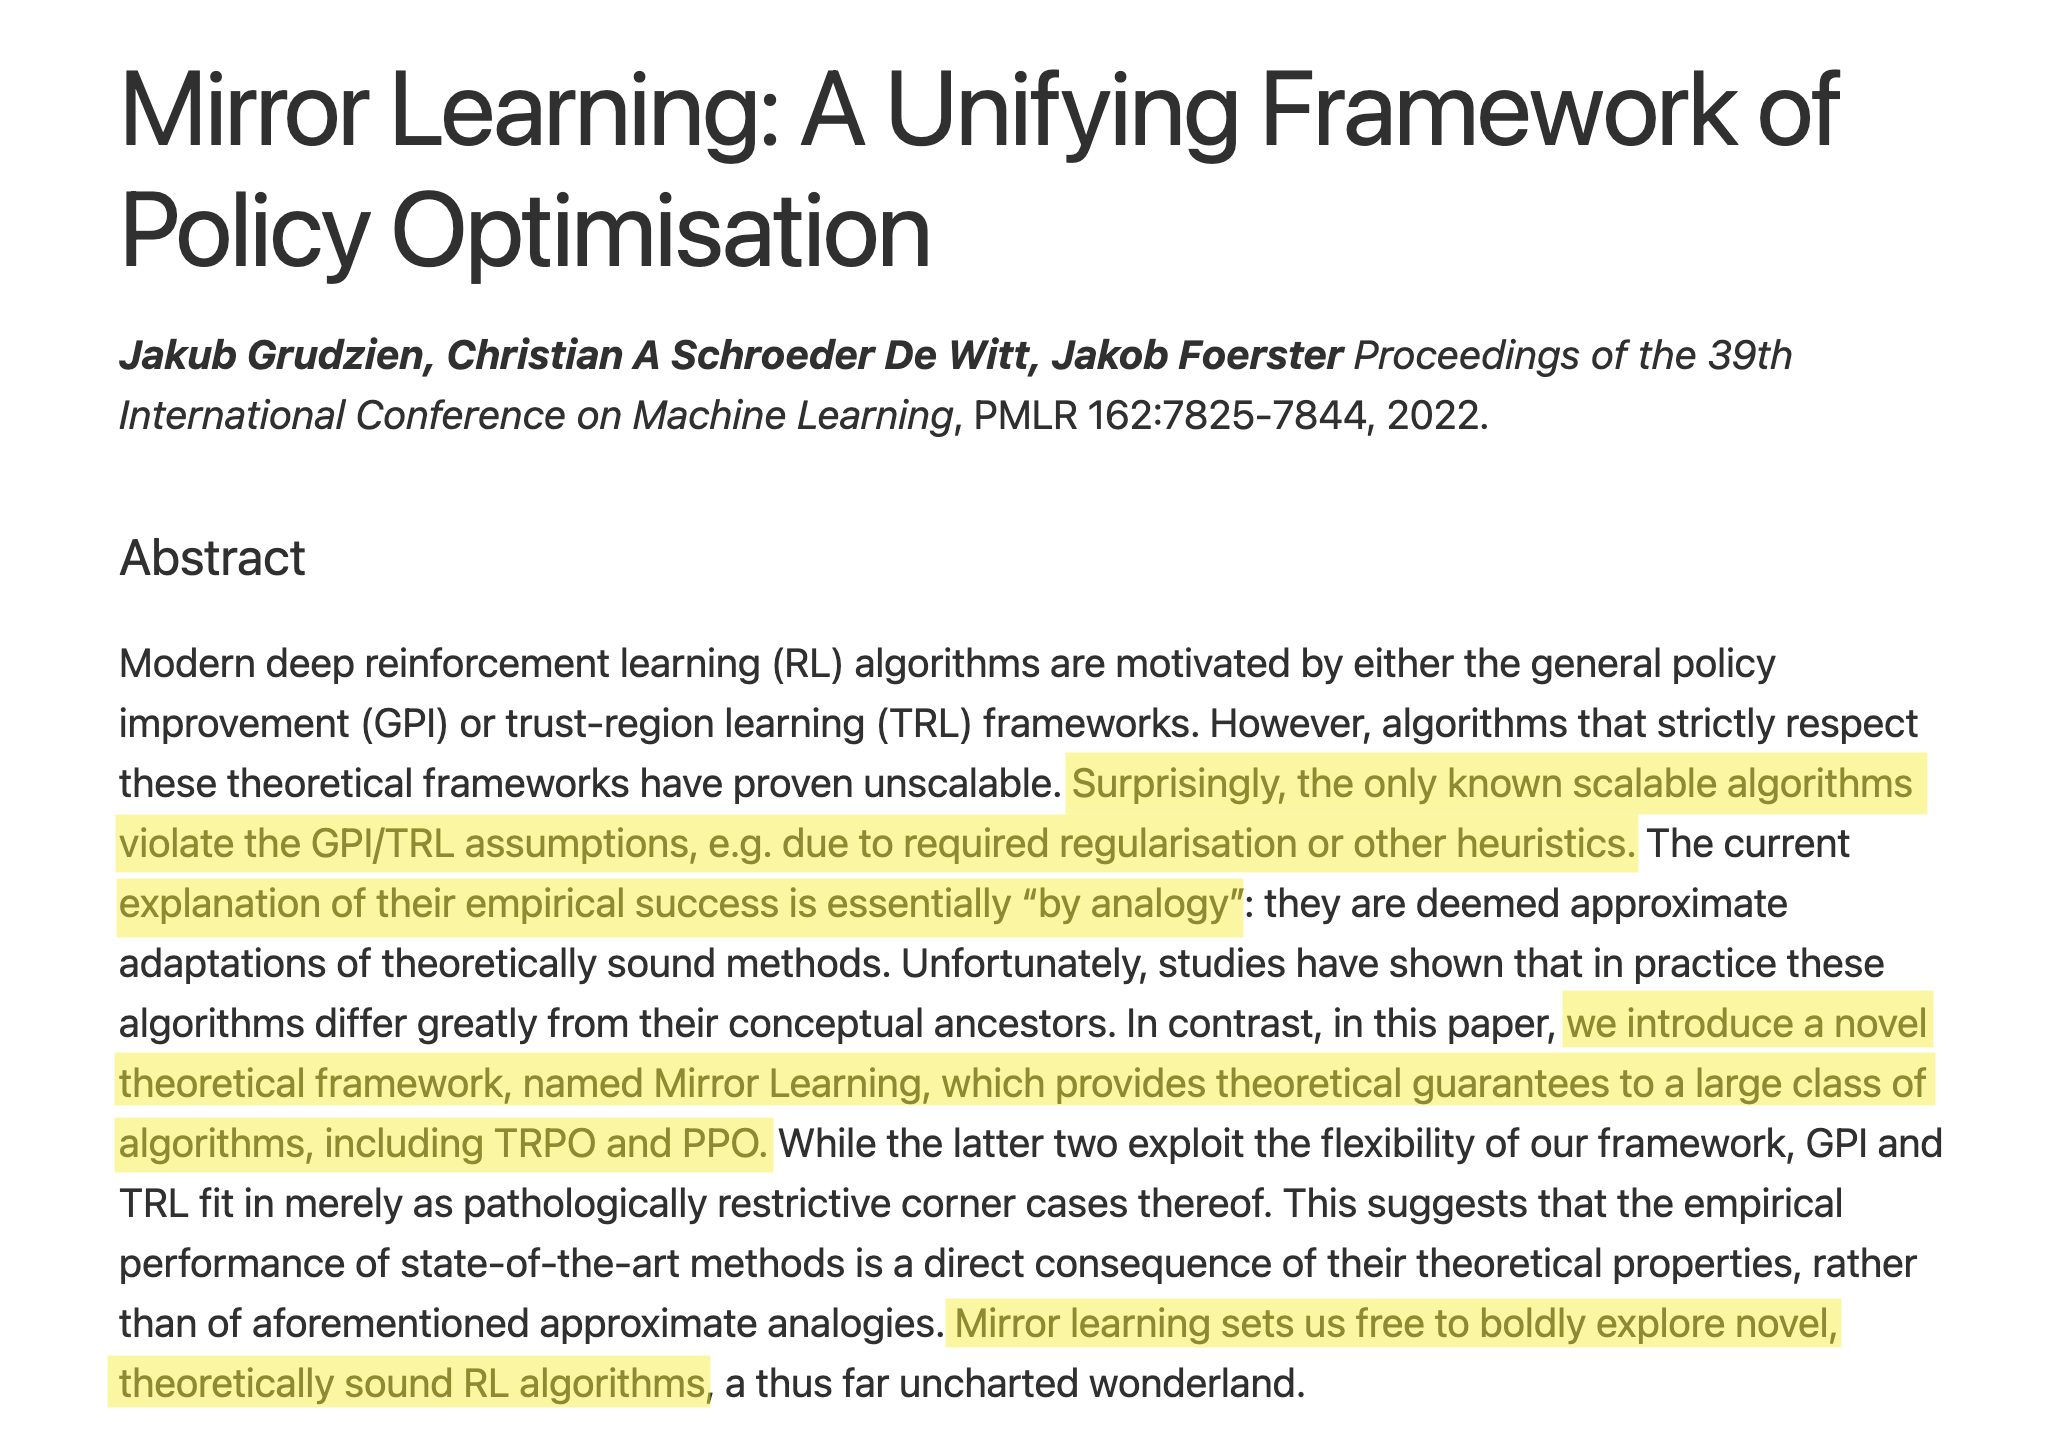
\includegraphics[width=0.85\textwidth]{figures/mirror_learning.png}
    \caption{Mirror Learning paper \cite{mirror2022}.}
    \label{fig:trl1}
  \end{figure}
\end{frame}


\begin{frame}{Mirror Learning (cont.)}
  \begin{block}{Mirror Learning Update}
  \begin{equation}
    \pi_{i+1} = \arg \max_{\pi' \in \mathcal{N}(\pi_i)} \mathbb{E}_{s \sim \pi_i} \left[ A_{\pi_i}(s, a) \right] - \mathcal{D}_{\pi_i}(\pi'),
  \end{equation}
  \end{block}
  
    \vspace{1em}  % Adds space between points for better distribution
  \begin{itemize}
    \item \( \mathcal{N}(\pi_i) \): The neighborhood of the current policy \( \pi_i \), which defines the region around the policy in which the update is allowed.
    \vspace{1em}  % Adds space between points for better distribution
    \item \( \mathcal{D}_{\pi_i}(\pi') \): The drift function, which measures the "distance" or cost of updating the current policy \( \pi_i \) to the new policy \( \pi' \).
  \end{itemize}
\end{frame}

\begin{frame}{Mirror Learning (cont.)}
  \begin{block}{The Fundamental Theorem of Mirror Learning}
    \vspace{1em}  % Adds space between points for better distribution
    If the drift function satisfies the following conditions:
    \begin{itemize}
      \item \textbf{Non-negativity}: \( \mathcal{D}_{\pi_i}(\pi) \geq 0 \) for all policies \( \pi \) and \( \pi_i \),
      \item \textbf{Zero drift at current policy}: \( \mathcal{D}_{\pi_i}(\pi_i) = 0 \),
      \item \textbf{Zero gradient at current policy}: \( \nabla_{\pi_i} \mathcal{D}_{\pi_i}(\pi_i) = 0 \), the gradient of the drift function is zero when \( \pi = \pi_i \), i.e., "gentle" for small changes.
    \end{itemize}
    \vspace{1em}  % Adds space between points for better distribution
    Then the Mirror Learning algorithm attains the monotonic improvement property \( \eta(\pi_{i+1}) \geq \eta(\pi_i) \) and as \( i \to \infty \), \( \eta(\pi_i) \to \eta(\pi^*) \). \cite{mirror2022}.
    \vspace{1em}  % Adds space between points for better distribution
  \end{block}
\end{frame}



\begin{frame}{Mirror Learning \& GPI}
  \begin{block}{(Reminder) Mirror Learning Update}
    \vspace{1em}  % Adds space between points for better distribution
    \[
    \pi_{i+1} = \arg \max_{\pi' \in \mathcal{N}(\pi_i)} \mathbb{E}_{s \sim \pi_i, a \sim \pi'} \left[ A_{\pi_i}(s, a) \right] - \mathcal{D}_{\pi_i}(\pi'),
  \]
    \vspace{1em}  % Adds space between points for better distribution
  \end{block}
  
  \begin{block}{Generalized Policy Iteration}
    \vspace{1em}  % Adds space between points for better distribution
  If we set \( \mathcal{D}_{\pi_i}(\pi) \equiv 0\) and \(\mathcal{N}(\pi_i) \equiv \Pi\) we obtain:
\[
    \pi_{i+1} = \arg \max_{\pi' \in \Pi} \mathbb{E}_{s \sim \pi_i, a \sim \pi'} \left[ A_{\pi_i}(s, a) \right] - 0,
    \]
\pause
  Which is equivalent to General Policy Iteration (GPI) update:
\[
    \pi_{i+1} = \arg \max_{\pi' \in \Pi} \mathbb{E}_{s \sim \pi_i, a \sim \pi'} \left[ Q_{\pi_i}(s, a) \right],
    \]
  Since \(A_{\pi_i}(s, a) = Q_{\pi_i}(s, a) - V_{\pi_i}(s)\)
    \vspace{1em}  % Adds space between points for better distribution
  \end{block}
  
\end{frame}

\begin{frame}{Mirror Learning \& PPO}

Recall that PPO update is theoretically defined as:
\[
  \pi_{i+1} = \arg \max_{\pi' \in \Pi} \mathbb{E}_{s \sim \pi_i, a \sim \pi'} \left[ L_{\text{CLIP}} \right]
\]
  where
  \[
    L_{\text{CLIP}} = \mathbb{E}_{a \sim \pi} \Bigg[ \min \Bigg( r(\pi') A_{\pi}(s, a), \, \text{CLIP}\Big(r(\pi'), 1 \pm \epsilon\Big) A_{\pi}(s, a) \Bigg) \Bigg].
\]
\pause
  By using the trick of "adding and subtracting" and importance sampling \( L_{CLIP} =\)
  \[
    \textcolor{blue}{\mathbb{E}_{a \sim \pi'} \Big[ A_\pi(s,a) \Big]} -\mathbb{E}_{a \sim \pi} \Bigg[ \textcolor{blue}{r(\pi')A_\pi(s,a)} - \min \Big( r(\pi') A_{\pi}(s, a), \, \text{clip}(r(\pi'), 1 \pm \epsilon) A_{\pi}(s, a) \Big) \Bigg].
\]

\pause
  Next, we focus on the expectation that is subtracted. First, we can replace the min operator with max, using the identity \( \min f(x) = \max [-f(x)] \), as follows:
  \[
    \mathbb{E}_{a \sim \pi} \Bigg[ \textcolor{black}{r(\pi')A_\pi(s,a)} - \max \Big(-r(\pi') A_{\pi}(s, a), \,-\text{clip}(r(\pi'), 1 \pm \epsilon) A_{\pi}(s, a) \Big) \Bigg].
\]

\end{frame}

\begin{frame}{Mirror Learning \& PPO (cont.)}

\[
    \mathbb{E}_{a \sim \pi} \Bigg[ \textcolor{blue}{r(\pi')A_\pi(s,a)} - \max \Big(\textcolor{blue}{-r(\pi') A_{\pi}(s, a)}, \,-\text{clip}(r(\pi'), 1 \pm \epsilon) A_{\pi}(s, a) \Big) \Bigg].
  \]

\pause
  Now, we move \textcolor{blue}{\( r(\pi) A_{\pi}(s, a) \)} inside the max, and obtain:
\[
    \mathbb{E}_{a \sim \pi} \Bigg[ \max \Big( \textcolor{blue}{0}, \Big[\textcolor{blue}{r(\pi')}-\text{clip}(r(\pi'), 1 \pm \epsilon) \Big]\textcolor{blue}{A_{\pi}(s, a)} \Big) \Bigg].
  \]
\pause

  Finally, we can simplify this as:
\[
    \mathbb{E}_{a \sim \pi} \Bigg[ \text{ReLU} \Big(\Big[r(\pi')-\text{clip}(r(\pi'), 1 \pm \epsilon) \Big]A_{\pi}(s, a) \Big) \Bigg].
  \]

\end{frame}


\begin{frame}{Mirror Learning \& PPO (cont.)}

  \begin{block}{Mirror Learning view of PPO}
    \vspace{1em}  % Adds space between points for better distribution
    \[
    \pi_{i+1} = \arg \max_{\pi' \in \Pi} \mathbb{E}_{s \sim \pi_i, a \sim \pi'} \left[ A_{\pi_i}(s, a) \right] - \mathcal{D}^{\text{PPO}}_{\pi_i}(\pi'),
  \]
  where
\[
    \mathcal{D}^{\text{PPO}}_{\pi_i} \equiv \mathbb{E}_{s \sim \pi_i, a \sim \pi'} \Bigg[ \text{ReLU} \Big(\Big[r(\pi')-\text{clip}(r(\pi'), 1 \pm \epsilon) \Big]A_{\pi}(s, a) \Big) \Bigg].
  \]
    \vspace{1em}  % Adds space between points for better distribution
  \end{block}

    \pause
  \begin{block}{Monotonic improvement of PPO}
    To show monotonic improvement property, it suffices to show that:
    \begin{itemize}
      \item \textbf{Non-negativity}: \( D^{\text{PPO}}_{\pi_i}(\pi) \geq 0 \) for all policies \( \pi \) and \( \pi_i \),
      \item \textbf{Zero drift at current policy}: \( D^{\text{PPO}}_{\pi_i}(\pi_i) = 0 \),
      \item \textbf{Zero gradient at current policy}: \( \nabla_{\pi_i} \mathcal{D}_{\pi_i}(\pi_i) = 0 \), the gradient of the drift function is zero when \( \pi = \pi_i \), i.e., "gentle" for small changes.
    \end{itemize}
  \end{block}
\end{frame}


\begin{frame}{Mirror Learning Space}
  \begin{flushleft} % Aligns the text to the left
    \begin{itemize}

      \item \textbf{Mirror Learning reveals more algorithms}
                \hfill
        \begin{itemize}
          \item An infinite space of theoretically sound mirror learning algorithms beyond PPO.
        \end{itemize}
        \begin{itemize}
          \item It is sufficient that proper conditions of the drift functions are satisfied.
        \end{itemize}

          \hfill
      \item \textbf{Current algorithms are handcrafted}
                \hfill
        \begin{itemize}
          \item PPO and others were handcrafted through intuition \& trial and error, and may not be optimal for learning.
        \end{itemize}
    
    \end{itemize}
  \end{flushleft}

  \hfill
  \begin{figure}

    \centering
    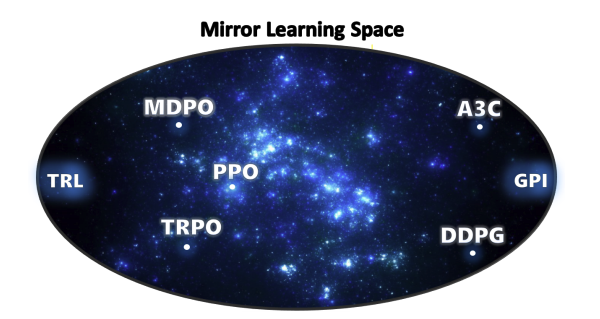
\includegraphics[width=0.7\textwidth]{figures/mirror_space.png}  % Replace this with your actual image path
    \caption{Taken from \cite{mirror2022}.}

  \end{figure}
\end{frame}



\begin{frame}[plain]
  \section{Disovered Policy Optimisation}
  \vfill
  \begin{center}
    \Huge \textbf{Disovered Policy Optimisation}
  \end{center}
  \vfill
\end{frame}

\begin{frame}{Meta-Learning}

    \vspace{1em}  % Adds space between points for better distribution
    \begin{itemize}
      \item \textbf{"Learning to learn"}: Find the best learning algorithm for a distribution of tasks.
        \pause
    \vspace{1em}  % Adds space between points for better distribution
        \item \textbf{Outer loop}: Optimizes the learning algorithm.
    \vspace{1em}  % Adds space between points for better distribution
        \item \textbf{Inner loop}: Optimizes the model parameters.
    \vspace{1em}  % Adds space between points for better distribution
    \end{itemize}
        \pause
  \begin{figure}
    \centering
    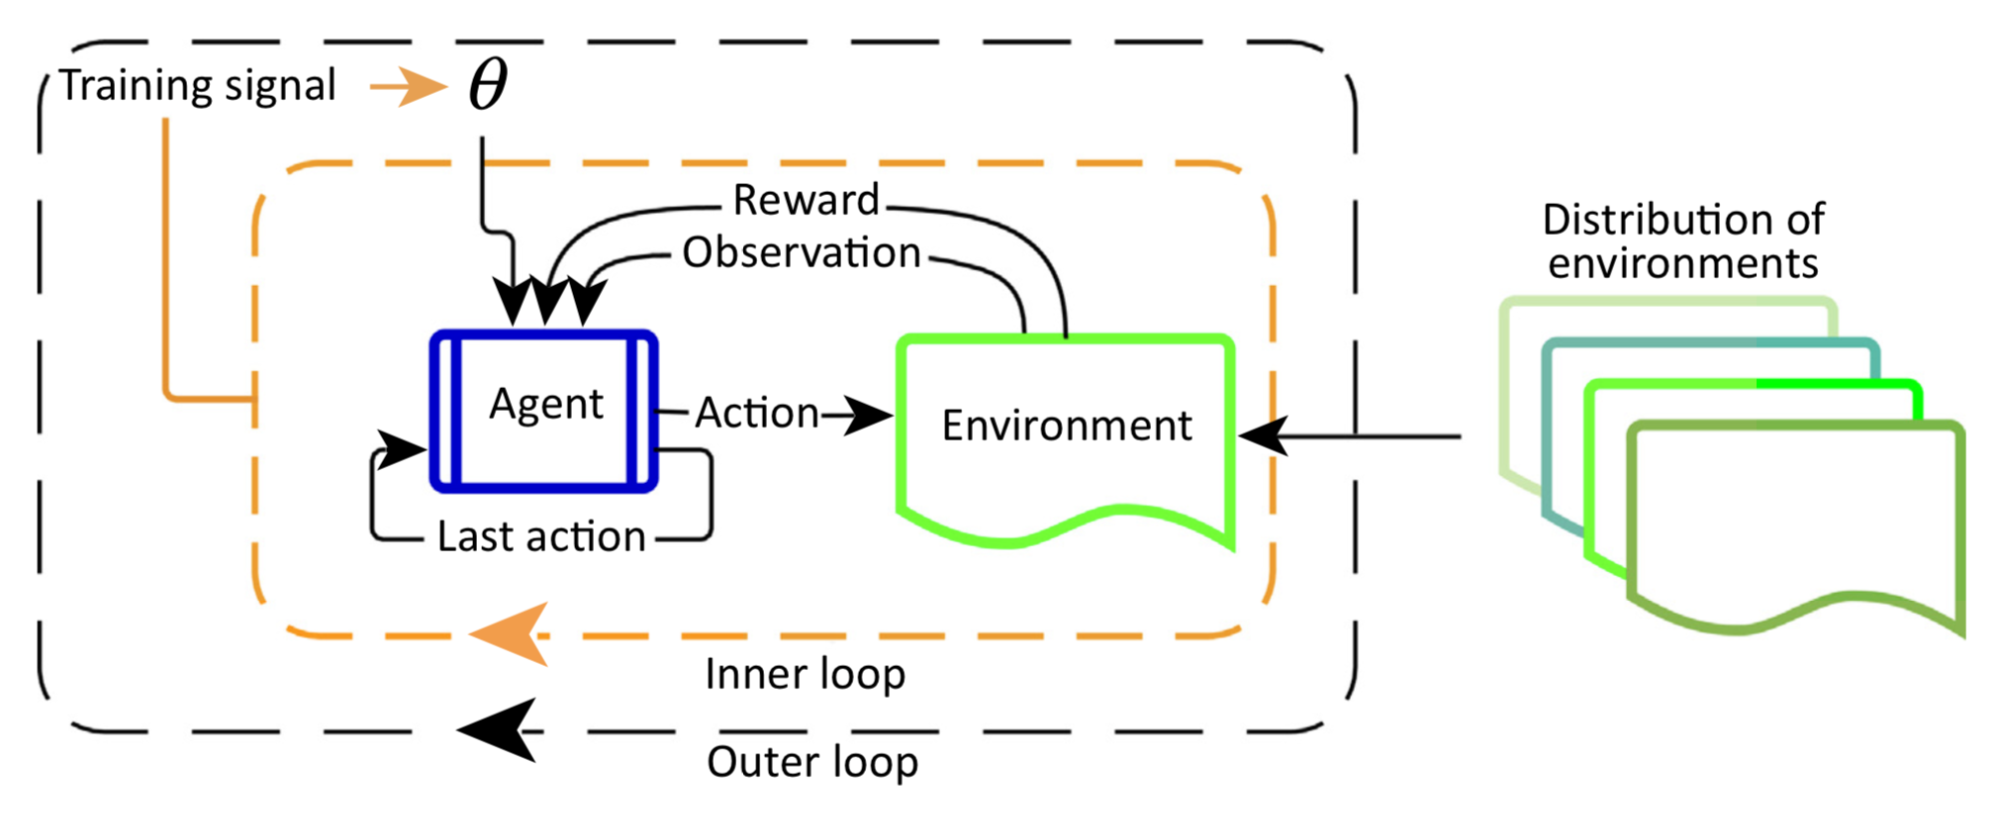
\includegraphics[width=0.9\textwidth]{figures/meta-learning.png}
    \caption{Meta-RL training loops \cite{weng2019meta}.}
    \label{fig:trl2}
  \end{figure}

\end{frame}


\begin{frame}{Mirror Learning + Meta-learning = DPO}
  \begin{figure}
    \centering
    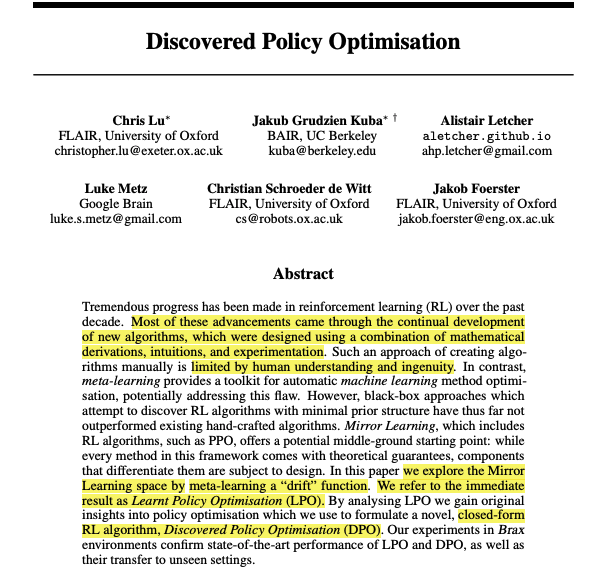
\includegraphics[width=0.65\textwidth]{figures/dpo_paper.png}
    \caption{Discovered Policy Optimisation paper \cite{dpo2022}.}
    \label{fig:trl3}
  \end{figure}
\end{frame}


\begin{frame}{Learnt Policy Optimization (LPO)}

\begin{itemize}
    \vspace{1em}  % Adds space between points for better distribution
  \item Use meta-learning to learn the optimal\footnote{Optimal w.r.t. the distribution of the tasks.} drift function \( \mathcal{D}^*_{\pi_i}(\pi') \).
    \vspace{1em}  % Adds space between points for better distribution
    \pause
  \item The drift function is approximated using a neural network computing function \( f \) with parameters \( \phi \) and input \( x \).
  \[
    \mathcal{D}_{\pi_i}(\pi') \approx \mathbb{E}^{\pi_i}\big[f_\phi(x)\big]
  \]
  
\end{itemize}

\end{frame}


\begin{frame}{LPO Network}

  On input \(f\) receives probability ratio between a candidate and the old policy, defined as:
  \(
  r = \frac{\pi'(a|s)}{\pi(a|s)},
  \)
  the advantage:
  \(
  A = A_{\pi}(s, a),
  \)

    \vspace{1em}  % adds space between points for better distribution
  
  \pause
  
  To ease learning complicated mappings, apply non-linear transformations of the arguments (as shown in E), forming the following input:

  \[
  x_{r, A} = \left[ (1 - r), (1 - r)^2, (1 - r)A, (1 - r)^2 A, \log(r), \log(r)^2, \log(r)A, \log(r)^2 A \right]
  \]

  \pause

  In order to guarantee that the neural network is a valid drift function, it must satisfy:
  \begin{itemize}
    \item \( f_\phi(x_{r,A}) = 0 \) and \( \nabla_r f_\phi(x_{r,A}) = 0 \) whenever \( r = 1\ (\pi=\pi')\),
    \item \( f_\phi(x_{r,A}) \geq 0 \) everywhere.
  \end{itemize}
    \vspace{1em}  % adds space between points for better distribution

  \pause

  In this model, \( x_{r,A} = 0 \) whenever \( r = 1 \), and the first condition is guaranteed by excluding bias terms from the network architecture.

  \pause
  
  To meet the latter two conditions, we apply the ReLU activation at the last layer with a slight shift:
  \[
  x \mapsto \text{ReLU}(x - \xi), \quad \xi = 10^{-6}
  \]
\end{frame}

\begin{frame}{LPO Training Loop}

  \begin{itemize}
    \item \textbf{Inner loop}:
      Train the model by optimizing the model parameters \( \theta \).

    \vspace{1em}  % Adds space between points for better distribution
    \item \textbf{Outer loop}:
      Estimate the gradient and update the meta-parameters \( \phi \) using Evolution Strategies (ES).
      \begin{itemize}
    \vspace{1em}  % Adds space between points for better distribution
        \item ES approximates the gradient by sampling random perturbations \( \epsilon \) and evaluating the objective function at \( \phi + \sigma \epsilon \).
    \vspace{1em}  % Adds space between points for better distribution
        \item This approach eliminates the need for back-propagation
      \end{itemize}
  \end{itemize}
  \begin{figure}
    \centering
    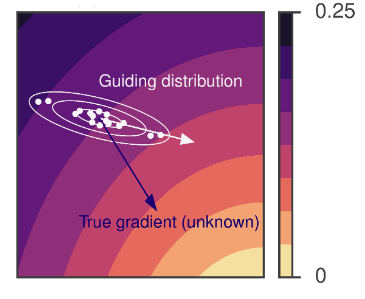
\includegraphics[width=0.35\textwidth]{figures/es.png}
    \caption{Gradient estimation using ES \cite{maheswaranathan2019guided}.}
    \label{fig:trl4}
  \end{figure}
\end{frame}


\begin{frame}{LPO technical details}

  \begin{itemize}
    \item Two variants trained
    \vspace{1em}  % Adds space between points for better distribution
  \begin{itemize}
    \item LPO-Zero: trained from scratch
    \vspace{1em}  % Adds space between points for better distribution
    \item LPO: adding \textcolor{blue}{PPO's drift} at the last layer 
    \[
   f_\phi(x_{r, A}) = \text{ReLU}\left( \tilde{f}_\phi(x_{r, A}) - \xi + \textcolor{blue}{\text{ReLU} \left( \left( r - \text{clip}(r, 1 \pm \epsilon) \right) \cdot A \right)} \right)
    \]
    where \( \tilde{f}_\phi(x_{r, A}) \) is the output of the last hidden layer of the drift network.
    \vspace{1em}  % Adds space between points for better distribution
  \end{itemize}
    
    \item Drift function neural network with 1 hidden layer and 128 hidden units
    \vspace{1em}  % Adds space between points for better distribution
    \item Default hyperparameters for PPO
    \vspace{1em}  % Adds space between points for better distribution
    \item 4 V100 GPUs
    \vspace{1em}  % Adds space between points for better distribution
    \item ~700 outer iterations \( \approx \) 2 days of compute
  \end{itemize}
  
\end{frame}


\begin{frame}{LPO findings}
  \begin{figure}
    \centering
    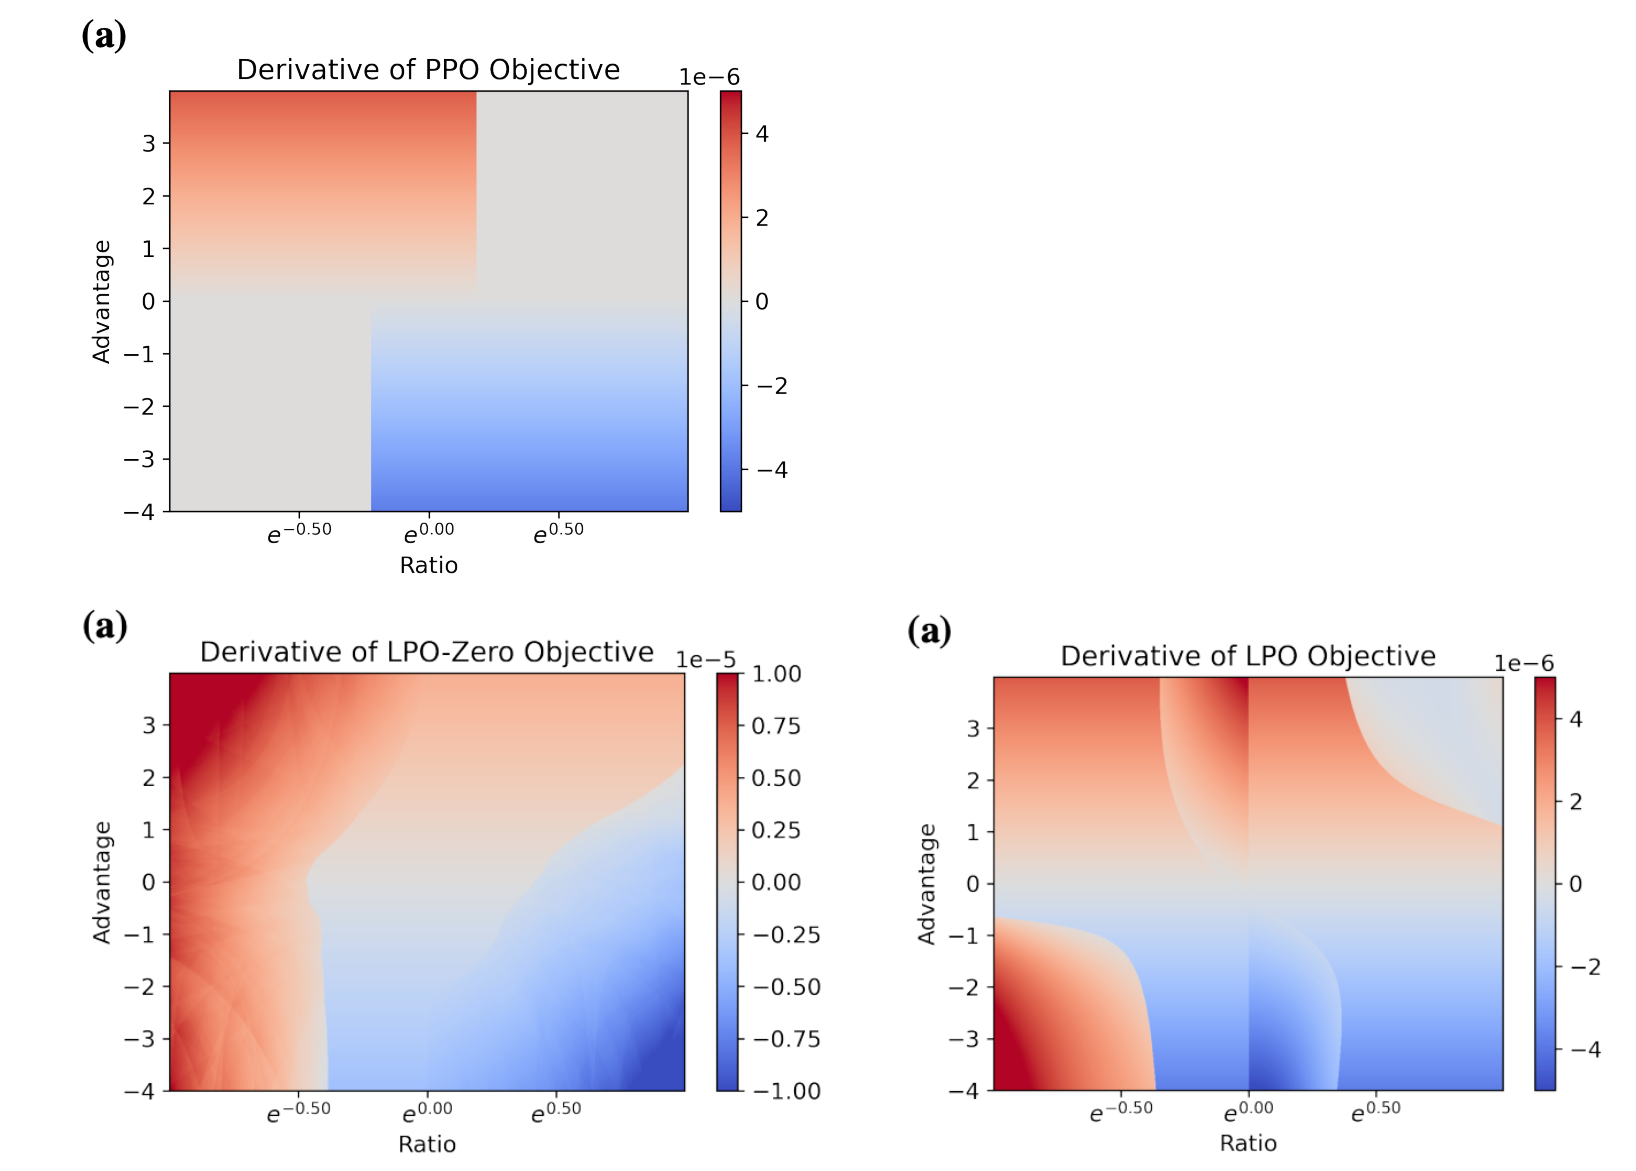
\includegraphics[width=0.8\textwidth]{figures/results1.png}
    \caption{Derivative of the Objective for PPO, LPO-Zero, and LPO \cite{dpo2022}.}
    \label{fig:trl5}
  \end{figure}
\end{frame}


\begin{frame}{From LPO to DPO}

  \begin{itemize}
    \item A closed-form formula would be much better than a neural network!
    \begin{equation}
  f_{\text{DPO}}(r, A) = \begin{cases} 
    \text{ReLU}\left( (r - 1)A - \alpha \tanh\left(\frac{(r - 1)A}{\alpha}\right) \right) & \text{if } A \geq 0, \\
    \text{ReLU}\left( \log(r)A - \beta \tanh\left( \frac{\log(r)A}{\beta} \right) \right) & \text{if } A < 0.
  \end{cases}
\end{equation}
    \item For \( \alpha = 2 \) and \( \beta = 0.6 \), the formula reproduces key features of LPO.

  \begin{figure}
    \centering
    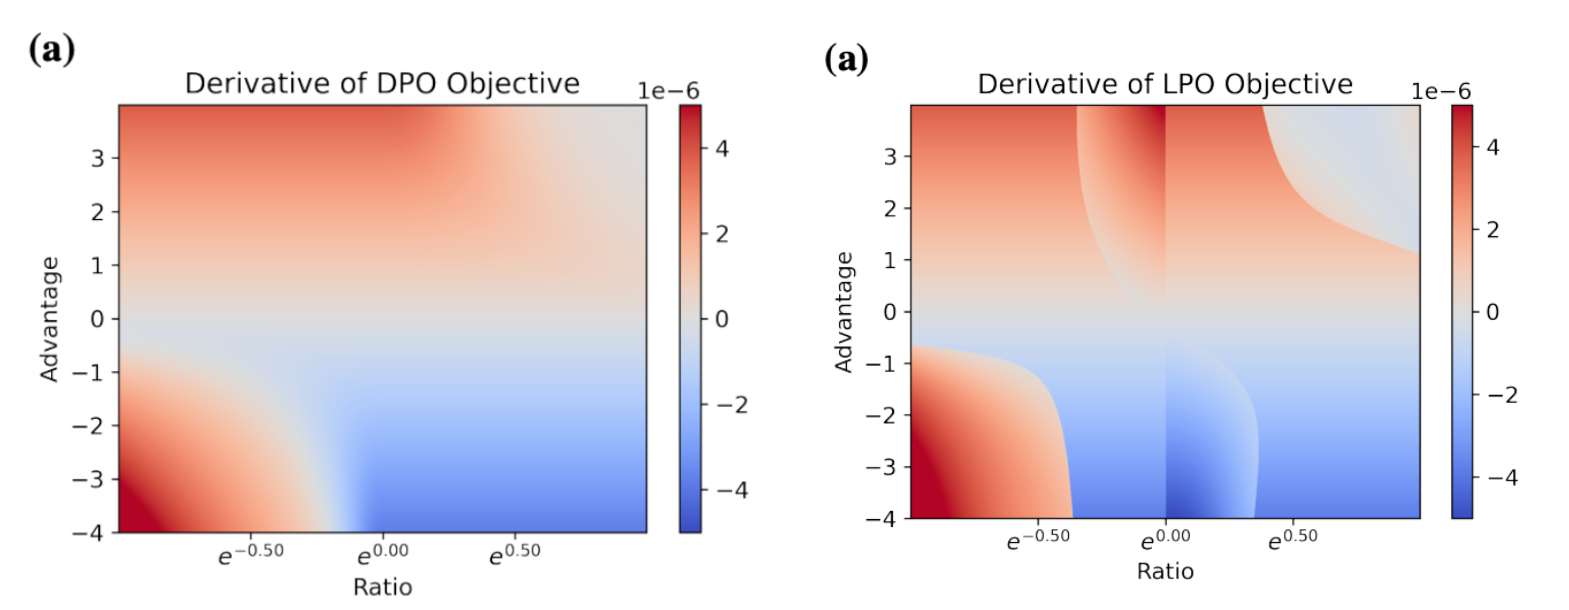
\includegraphics[width=0.8\textwidth]{figures/results2.png}
    \caption{Derivative of the Objective for DPO and LPO \cite{dpo2022}.}
    \label{fig:trl6}
  \end{figure}
  \pause
  
    \item Moreover, the formula satisfies the drift function properties \cite{dpo2022}, as a bonus, it is two lines of code update of PPO to integrate into RL libraries!
  \end{itemize}

\end{frame}

\begin{frame}{Evaluation}

  \begin{figure}
    \centering
    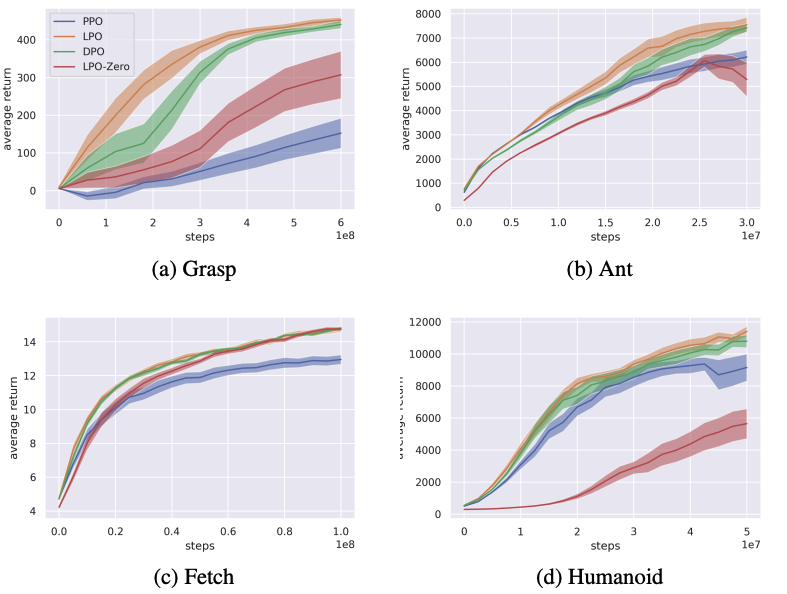
\includegraphics[width=0.75\textwidth]{figures/results3_plots.png}
    \caption{LPO, DPO, PPO performance comparison \cite{dpo2022} on Brax \cite{brax2021github} environments (10 seeds).}
    \label{fig:trl7}
  \end{figure}

\pause
  \begin{itemize}
    \item Note: LPO was meta-trained on a single environment (ant) only!
\end{itemize}
\vfill

\end{frame}

\begin{frame}{Evaluation (cont.)}

  \begin{figure}
    \centering
    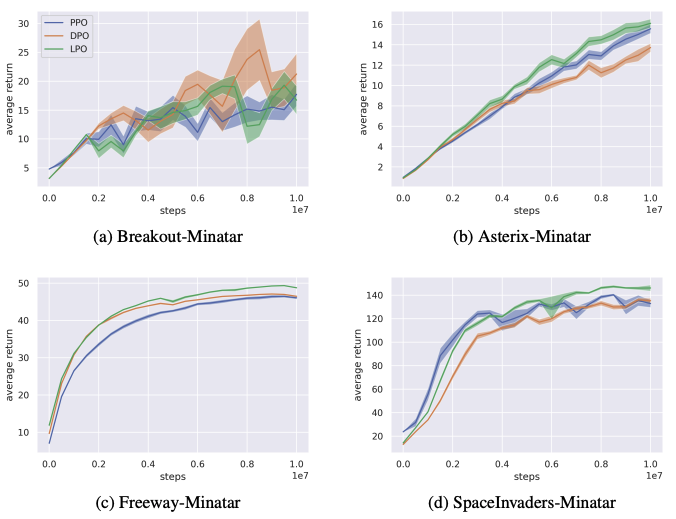
\includegraphics[width=0.8\textwidth]{figures/minatar.png}
    \caption{LPO, DPO, PPO performance comparison \cite{dpo2022} on Minatar \cite{young19minatar} environments (10 seeds).}
    \label{fig:trl8}
  \end{figure}

\end{frame}
\begin{frame}{Evaluation (cont.)}

  
    \vfill
  \begin{itemize}
    \item Both LPO and DPO outperform PPO on tasks they were not meta-learned for.
    \vfill
    \item Moreover, they use default PPO's finetuned hyperparameters for the given task.
    \vfill
    \pause
    \item Both LPO and DPO show both greater stability, possibly due to better exploration \cite{dpo2022}.
\end{itemize}
    
    \vfill
  \begin{figure}
    \centering
    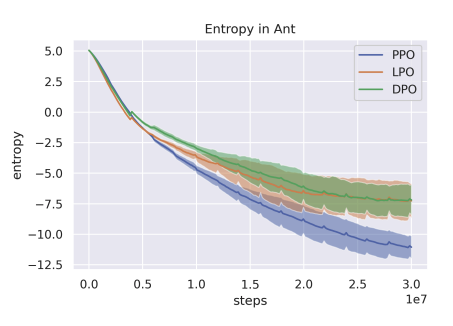
\includegraphics[width=0.5\textwidth]{figures/results4_entropy.png}
    \caption{Comparison of entropy between PPO, LPO, and DPO on ant environment \cite{dpo2022}.}
    \label{fig:trl9}
  \end{figure}

\end{frame}

\begin{frame}{Takeaways \& Future Work}

  \begin{itemize}
    \vfill
    \item \textbf{Key takeaways}:
  \begin{itemize}
      \item Mirror learning shows there is an infinite space of theoretically sound RL algorithms
      \vfill
      \pause
      \item This space can be searched and SOTA algorithms discovered not by handcrafting but through meta-learning.
  \end{itemize}

  \pause
    \vfill
    \item \textbf{Future directions}:
  \begin{itemize}
    \item Find the optimal drift function for each time-step.
    \vfill
    \pause
    
    \item LLM-guided Discovery?
    \vfill
  \end{itemize}
\end{itemize}

\end{frame}

\begin{frame}{LLM-guided Discovery! (2024)}

  \begin{figure}
    \centering
    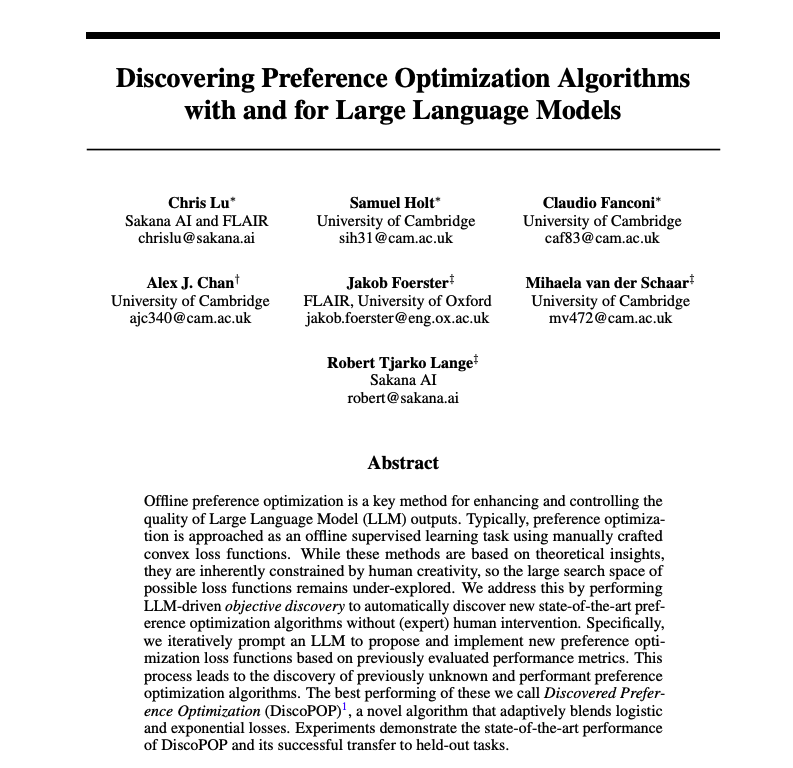
\includegraphics[width=0.6\textwidth]{figures/llm_disco.png}
    \caption{DPO follow-up paper \cite{lu2024discovering}.}
    \label{fig:trl10}
  \end{figure}
  
\end{frame}



\begin{frame}[t, allowframebreaks]{References}
\printbibliography[heading=none]
\end{frame}

\makeoutro

\end{document}